% Complete Section 4.3, original PDF 47-49 / printed 37-39.
% block: l2-de-rham-heading page:47 type:section
\subsection{{Example: The $L^2$ de Rham complex}}\label{sec:l2-de-rham-complex}

% block: l2-de-rham-base-domain page:47 type:ordinary-paragraph
{The prototypical example of a Hilbert complex is the de Rham complex associated to a Riemannian manifold. We continue to discuss the case of a domain $\Omega$ in $\mathbb R^3$, which we shall assume to have a Lipschitz boundary. The base Hilbert spaces will be $W^0=W^3=L^2(\Omega)$, $W^1=W^2=L^2(\Omega;\mathbb R^3)$. The operators are the ones discussed in Section~\ref{sec:vector-operators-adjoints}: $d^0=\operatorname{grad}$, $d^1=\operatorname{curl}$, $d^2=\operatorname{div}$, with the domains taken to be $H^1$, $H(\operatorname{curl})$, and $H(\operatorname{div})$, respectively. We saw there that these are closed operators, so we meet the criteria for a Hilbert complex. The domain complex, consisting of the spaces $V^k$, is}
\begin{equation}\label{eq:l2-de-rham-domain-complex}
0\to H^1\xrightarrow{\operatorname{grad}}H(\operatorname{curl})\xrightarrow{\operatorname{curl}}H(\operatorname{div})\xrightarrow{\operatorname{div}}L^2\to0.
\end{equation}

% block: l2-dual-domain-complex page:47 type:ordinary-paragraph
{In view of the adjoints computed in Section~\ref{sec:vector-operators-adjoints}, the domain complex of the dual complex (consisting of the $V_k^*$) is}
\begin{equation}\label{eq:l2-dual-domain-complex}
0\leftarrow L^2\xleftarrow{-\operatorname{div}}\mathring H(\operatorname{div})\xleftarrow{\operatorname{curl}}\mathring H(\operatorname{curl})\xleftarrow{-\operatorname{grad}}\mathring H^1\leftarrow0.
\end{equation}

% block: de-rham-compactness page:48 type:ordinary-paragraph
{An important fact is that the $L^2$ de Rham complex satisfies the compactness property, i.e., that $V^k\cap V_k^*$ is compactly included in $W^k$. For $k=0$, we have $V^0\cap V_0^*=H^1\cap L^2=H^1$ which is indeed compact in $W^0=L^2$ by Rellich's theorem. The result for $k=3$ is similar. For $k=1$ and $2$ the desired results are that $H(\operatorname{curl})\cap\mathring H(\operatorname{div})$ and $\mathring H(\operatorname{curl})\cap H(\operatorname{div})$ are compact in $L^2(\Omega;\mathbb R^3)$. This was proved, in the greater generality of Riemannian manifolds with Lipschitz boundary, by Picard \BookCite{62}. According to Theorem~\ref{thm:compactness-implies-fredholm}, the compactness property implies that the de Rham complex is Fredholm: the operators have closed range, and the harmonic form spaces are finite dimensional. In particular, we have established that $\operatorname{curl}H(\operatorname{curl})$ is closed, as claimed at the end of Chapter~\ref{chap:unbounded-operators}. We now calculate the spaces of harmonic forms and exhibit the Hodge decomposition for each degree.}

% block: harmonic-zero-forms page:48 type:ordinary-paragraph
{The space of harmonic $0$-forms coincides with $\mathcal Z^0$, the null space of the gradient. This is the space of constants, or, if we allow domains with more than the one connected component, the space of local constants. Its dimension is the number $b_0$ of connected components of $\Omega$ (the zeroth Betti number of the domain). Since the space $\mathcal B^0=0$, the Hodge decomposition expresses $L^2$ as the sum $\operatorname{div}\mathring H(\operatorname{div})$ and the constant (or locally constant) functions.}

% block: harmonic-one-forms pages:48,49 type:ordinary-paragraph
{The space of harmonic $1$-forms is more complicated. It consists of the $L^2$ vector fields $p$ for which $\operatorname{curl}p=0$, $\operatorname{div}p=0$, and the normal trace $\gamma_n p$ vanishes on $\partial\Omega$. An elementary example of such a function is pictured on the left of Figure~\ref{fig:de-rham-harmonic-fields}, in which the domain is an annular cylinder. In cylindrical coordinates the domain is given by $a\leq r\leq b$, $c\leq z\leq d$, for some $0<a<b$, $c<d$, and the harmonic forms are simply the multiples of $p=\operatorname{grad}\theta$. On a general domain $\dim\mathsf H^1=b_1$, the first Betti number, which we defined in Section~\ref{sec:simplicial-chain-complex} and which counts the number of tunnels through the domain. For a simply connected domain, $b_1=0$, and the Hodge decomposition is the classical Helmholtz decomposition of a vector field into a gradient (which is irrotational, meaning curl-free) and a curl (solenoidal, meaning divergence-free). For a general domain, we must also include the harmonic part:}
\[
L^2(\Omega;\mathbb R^3)=\operatorname{grad}H^1(\Omega)\BookOrthSum\operatorname{curl}\mathring H(\operatorname{curl};\Omega)\BookOrthSum\mathsf H^1.
\]

% block: de-rham-harmonic-fields-figure page:48 type:figure
\begin{figure}[htbp]\centering
\includegraphics[page=48,trim=89bp 83bp 57bp 445bp,clip,width=.85\linewidth]{../input/source/Finite Element Exterior Calculus.pdf}
\caption{{Left: Harmonic $1$-form on an annular cylinder in $\mathbb R^3$. Right: Harmonic $2$-form on a spherical shell (half the shell has been cut away for visibility).}}\label{fig:de-rham-harmonic-fields}
\end{figure}

% block: harmonic-two-forms page:49 type:ordinary-paragraph
{The space of harmonic $2$-forms consists of vector fields which are again curl- and divergence-free but, in this case, with vanishing tangential trace on the boundary. An elementary example is given in spherical coordinates on the closed spherical shell $a<r<b$ by $p=\operatorname{grad}(1/r)$. See Figure~\ref{fig:de-rham-harmonic-fields}. On a general domain, $\dim\mathsf H^2=b_2$, the number of voids in the domain. The Hodge decomposition is again into gradients and curls, but the boundary conditions are different, as is the space of harmonic forms:}
\[
L^2(\Omega;\mathbb R^3)=\operatorname{grad}\mathring H^1(\Omega)\BookOrthSum\operatorname{curl}H(\operatorname{curl};\Omega)\BookOrthSum\mathsf H^2.
\]

% block: harmonic-three-forms page:49 type:ordinary-paragraph
{Finally, the space of harmonic $3$-forms is simple: $\mathsf H^3=0$, since there are no nonzero functions in $\mathring H^1$ with vanishing gradient. Of course, $\mathcal B_3^*$ also vanishes, so the Hodge decomposition is trivial.}
